\documentclass{article}
\usepackage{multicol}
\usepackage{graphicx}
\usepackage[section]{placeins}
\usepackage{hyperref}
\hypersetup{
	colorlinks=true,
	linkcolor=blue,
	filecolor=magenta,      
	urlcolor=cyan,
}
\urlstyle{same}
\usepackage{caption}




\title{\Huge \bfseries \emph{Assignment 1}}
\author{Vathana Him}
\date{September 12, 2021}

\begin{document}
\maketitle

\begin{multicols}{2}
	
\section{Abstract}
	The purpose of this assignment was to begin the introduction to data preprocessing as a preparation step for machine learning and deep learning. This assignment utilized images from UCI respository as sample datasets that will be used to train a machine learning model. Images that were processed represented three fruits spanish pear, fuji apple, watermelon. 
	
	The data for these images were processed using the OpenCV python library. The main goals for this assignment were to process the data for each respective images into their appropriate feature space and feature vector, analyze thess datasets to see if there were any imbalance, explore if any standardization was needed, and export these data into appropriate .csv format to be used as training datasets for machine learning.  


\section{Setting Up}
The developing environment was installed by going to the anaconda website and downloading anaconda. Then anaconda was launched. Once it was launched, navigate to the environment tab, then the create button was pressed in order to create the new working environment. The enviroment was named as MSIA. Within the environment, python 3.7 was installed. Subsequently, pip was used to install a list of python libraries. These libraries included Opencv, Pandas, Plotly, Matplotlib, and Numpy.


\subsection{Section 1 Figures} 

	\begin{center}
		\captionof{figure}{environment}
		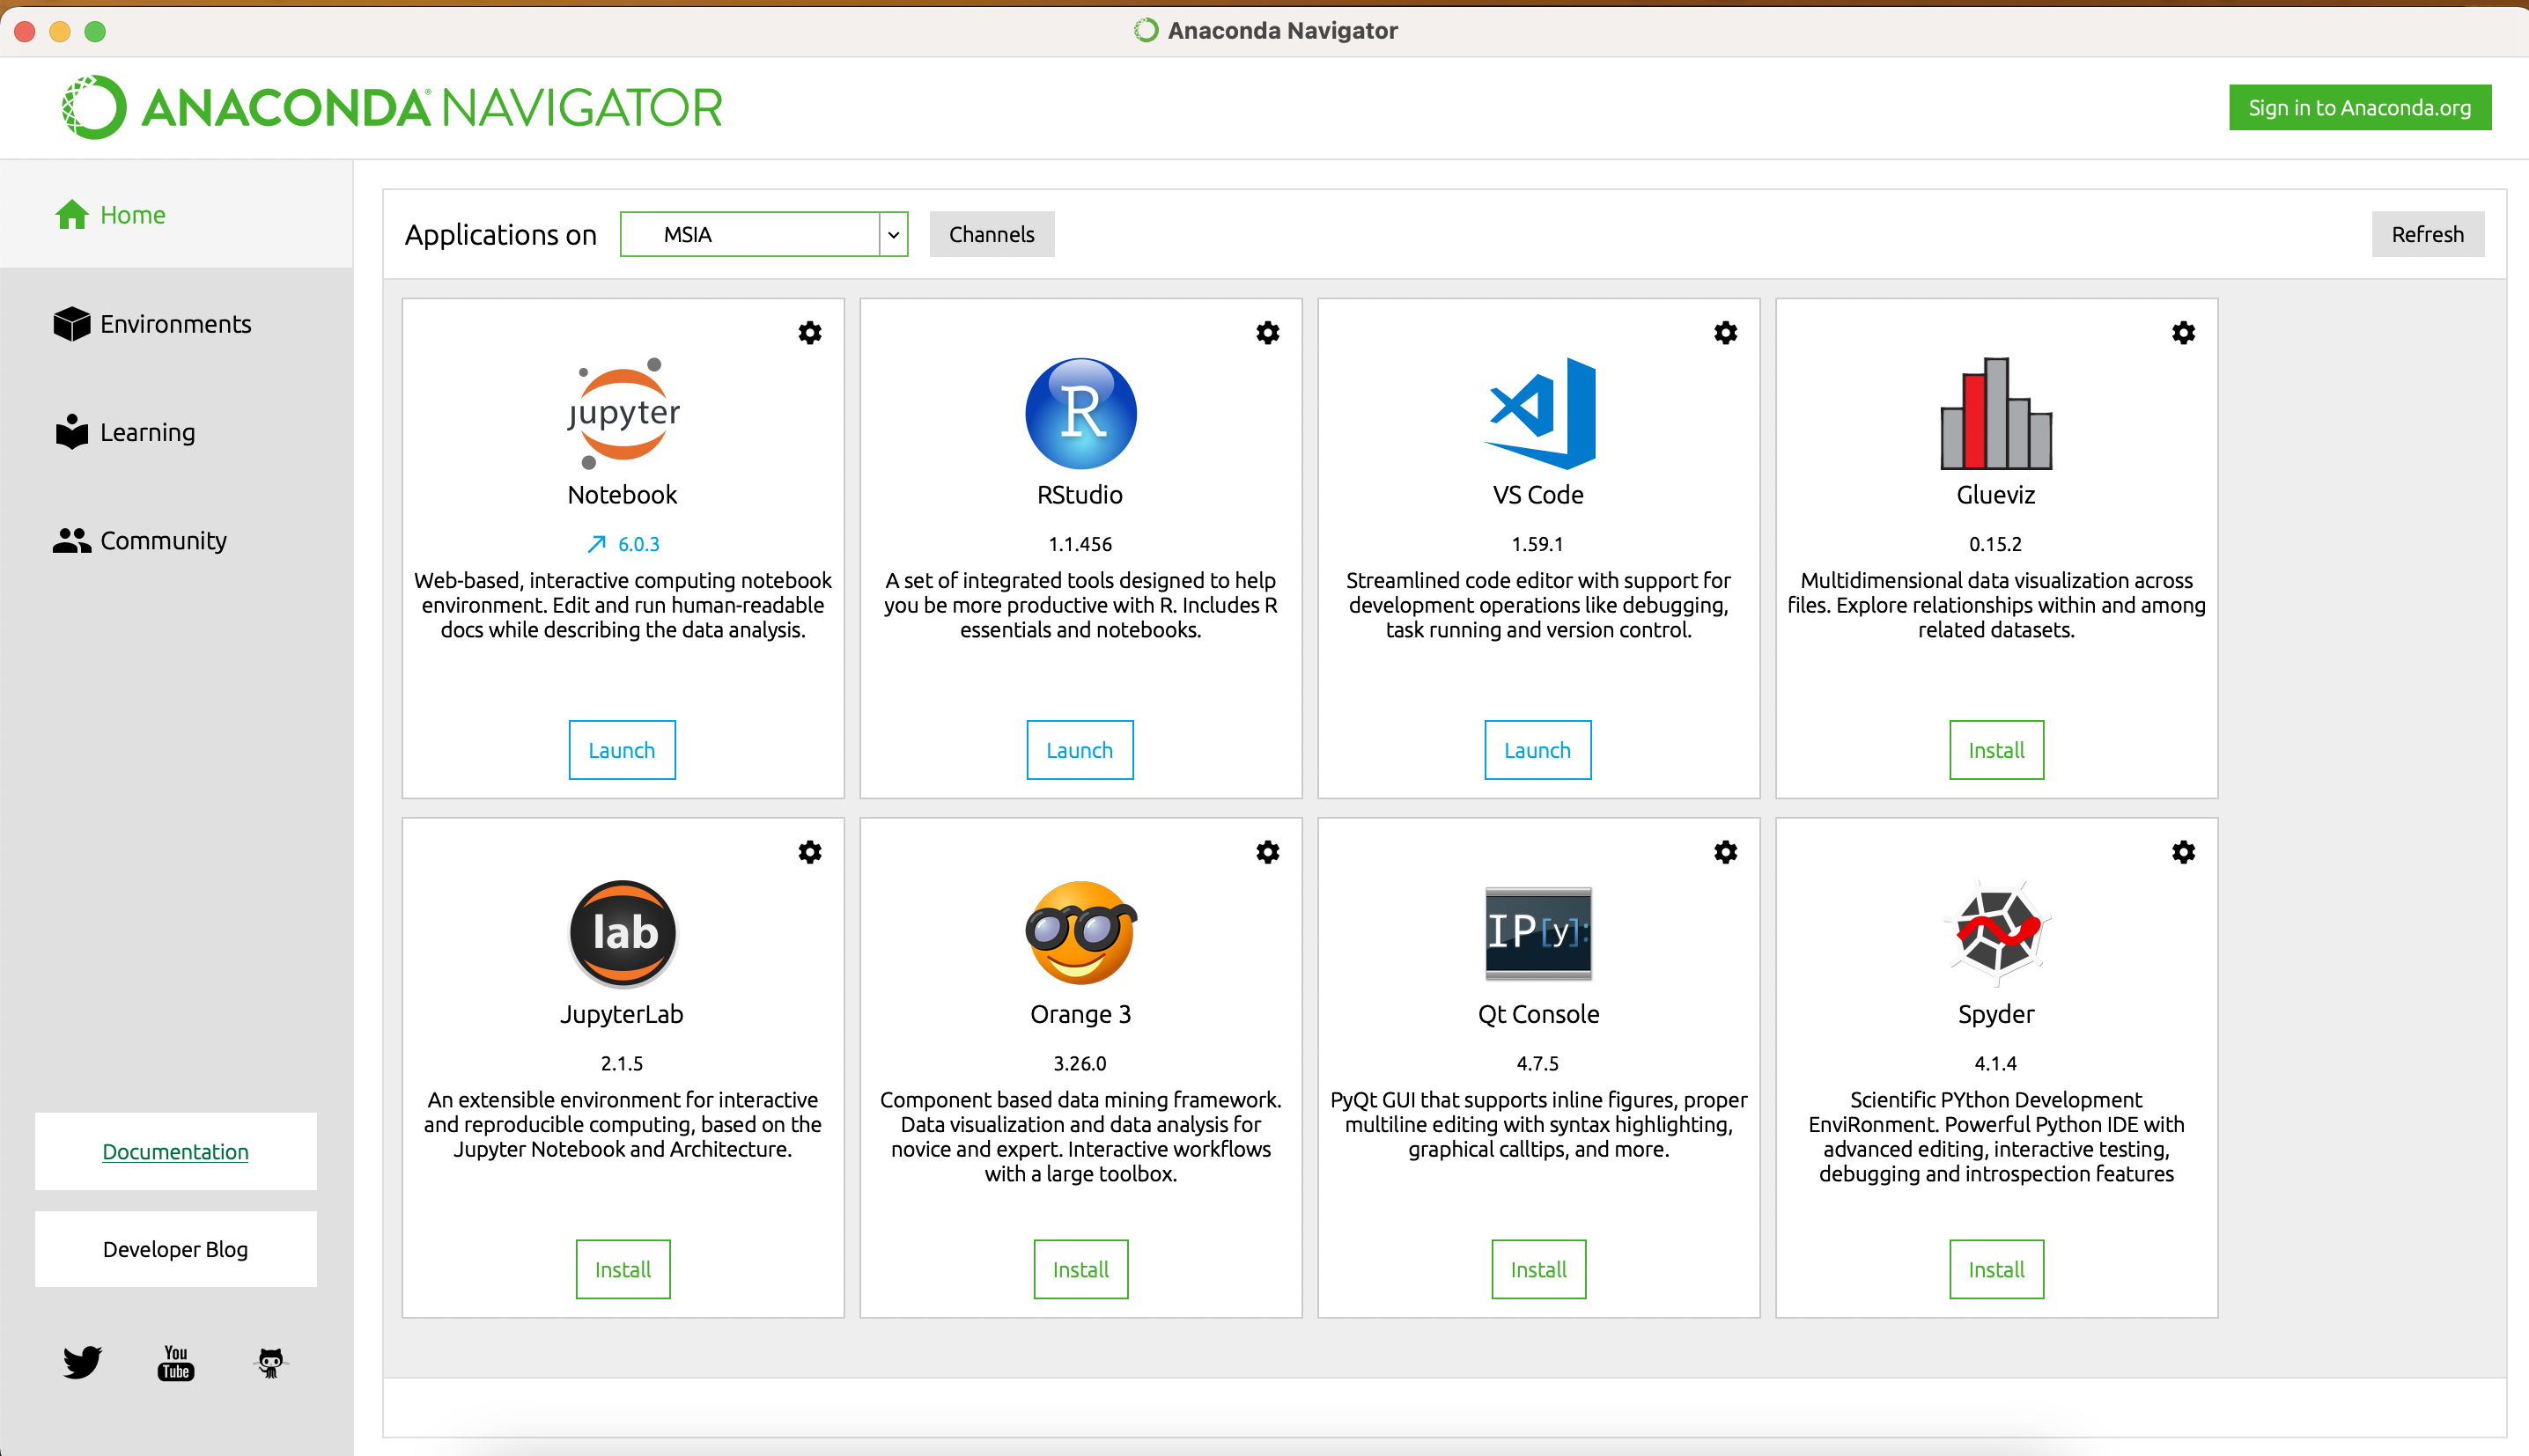
\includegraphics[scale=0.1]{../screenshots/environment.png}
		
	\end{center}

	\captionof{figure}{Pip Command}
	\begin{verbatim}
		Ex.
		pip install pandas
		pip install opencv
	\end{verbatim}
	

	

		
	

\section{Choosen Images}
The choosen images were gathered from the UCI data respository. The link for these images can be found \href{https://www.ic.unicamp.br/~rocha/pub/downloads/}{here} \footnote[1]{https://www.ic.unicamp.br/~rocha/pub/downloads/}. This dataset contains a variety of fruits and vegatables but only three images were choosen for this assignment. These image were spanish pear, fuji apple, and watermelon. Each of these images respresent a fuji apple, spanish pear,
and watermelon respectively. These images were chosen due to the nature of their color as apple was a bright red color, spanish pear was a bright yellow, and watermelon was green. Intuitively, the human eyes was able to distinguish the differences betweent these colors easily. In correlation, computer vision should be able to distinguish the same differences due to its difference in RGB value. Subsequently, these images also have consistent dimensions which makes scaling and resizing of images more consistent.


\subsection{Section 3 Figures} 
\centering
\captionof{figure}{Image Folders}
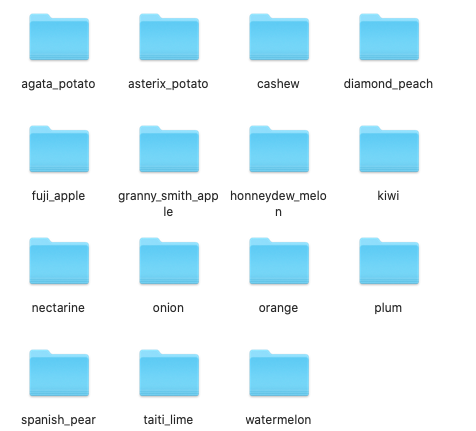
\includegraphics[scale=0.3]{../screenshots/image_folder.png}

\centering
\captionof{figure}{Spanish Pear}
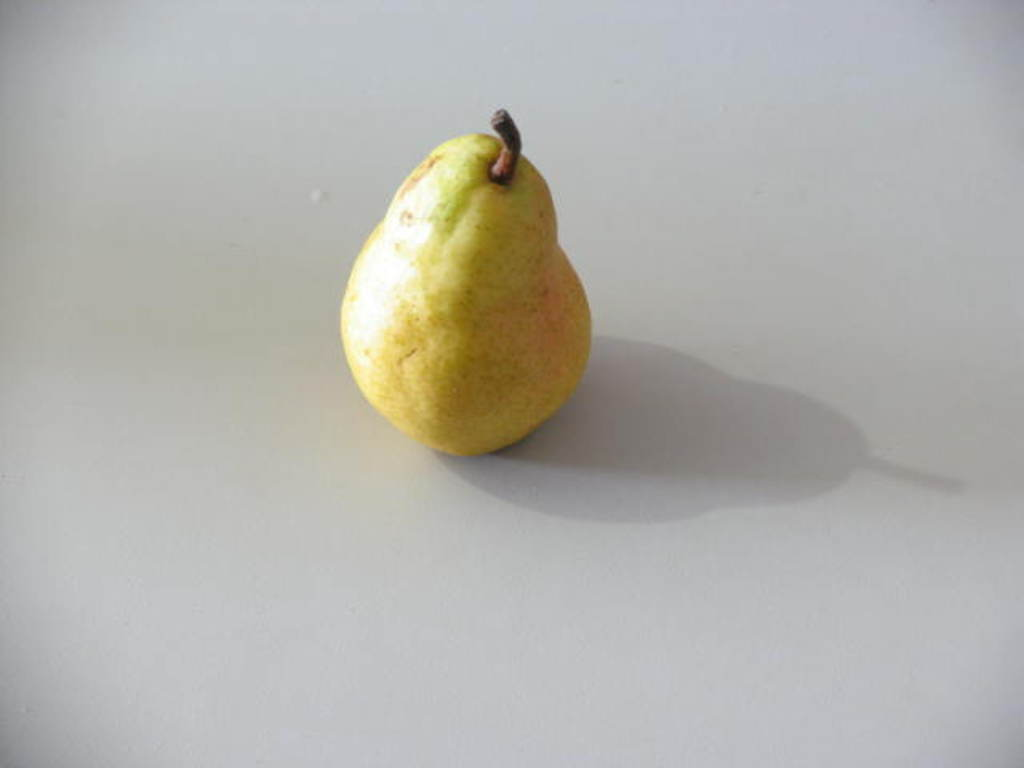
\includegraphics[scale=0.3]{../data/spanish_pear_001.jpg}

\centering
\captionof{figure}{Fuji Apple}
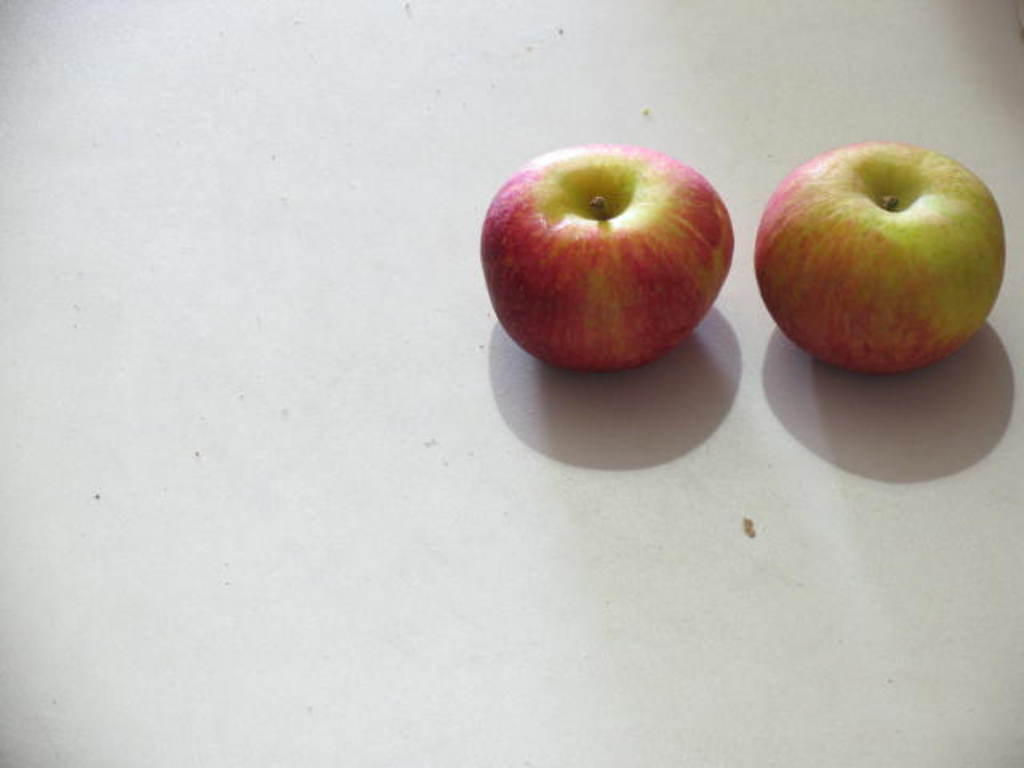
\includegraphics[scale=0.3]{../data/fuji_apple_001.jpg}

\centering
\captionof{figure}{Watermelon}
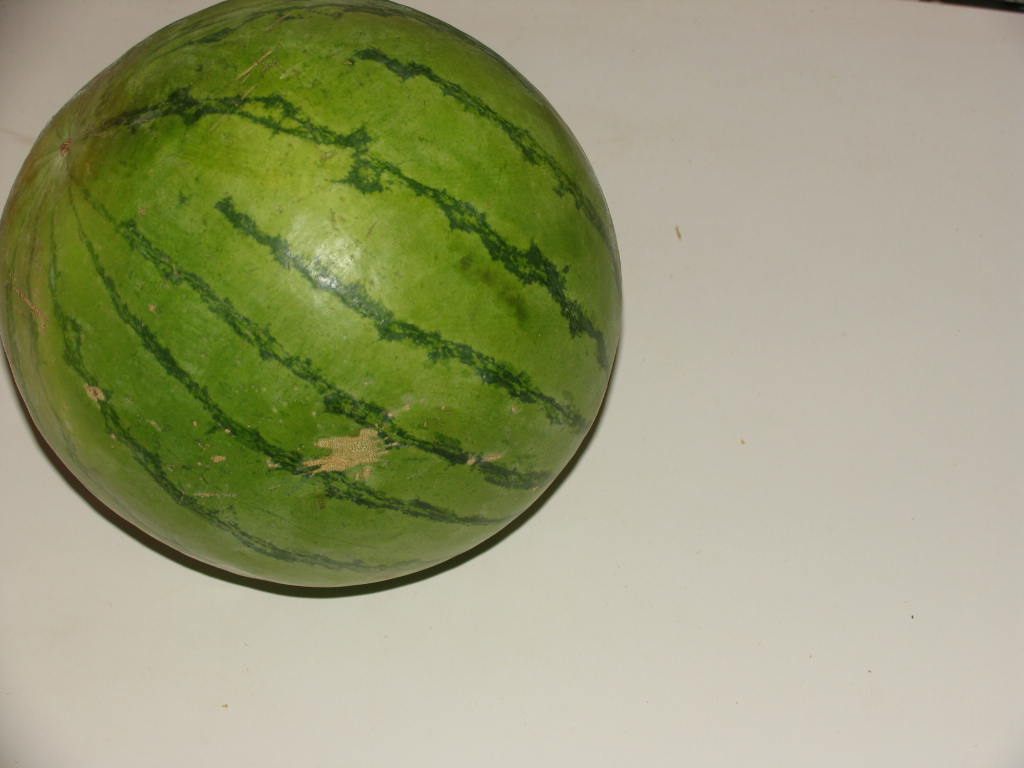
\includegraphics[scale=0.3]{../data/watermelon_001.jpg}




\end{multicols}

\end{document}